\documentclass{ximera}

\title{CoCalc}

%this is just a comment.
\begin{document}
\begin{abstract}
CoCalc is the easiest way for a new author to publish.
\end{abstract}
\maketitle

To publish your work to the internet, you will need a computer that
can run our tools. The developers of Ximera use \link[Arch Linux]{http://www.archlinux.org/}, but we believe that to be too difficult for the average user. Instead, we suggest you use \link[CoCalc]{http://cocalc.com/}.

Once you have a CoCalc account, you will need to start a new project

\begin{image}
  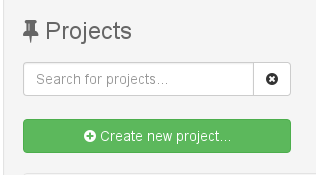
\includegraphics{createNewProject.png}
\end{image}

And when you create this new project, give it a Title, and a
Description. This project \textbf{must} have internet access.
\begin{image}
  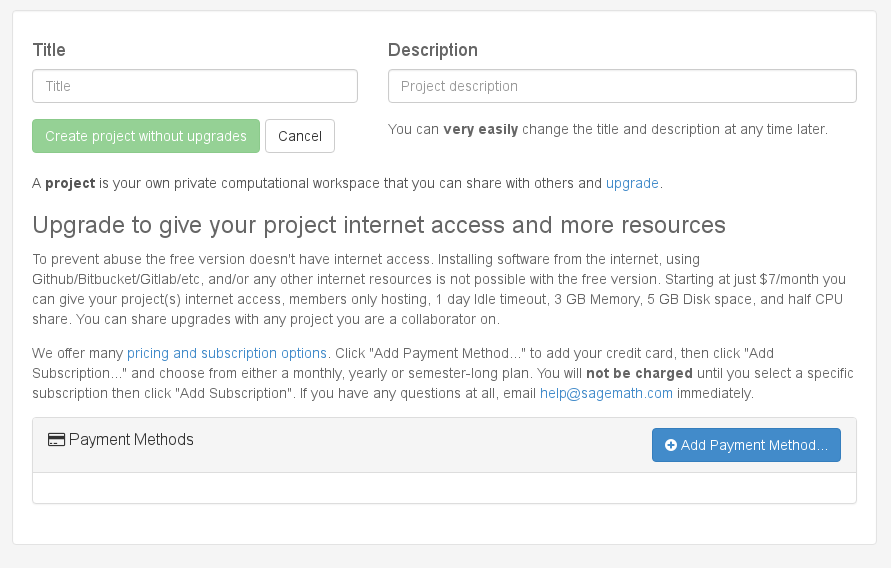
\includegraphics{internet.png}
\end{image}
Now you will need to add a terminal to your CoCalc account, click on
\begin{image}
  
\includegraphics{create.png}
\end{image}
and select ``Terminal.'' 
\begin{image}
  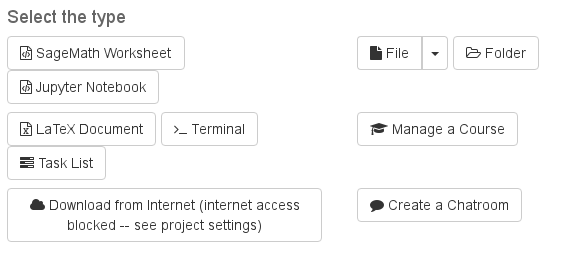
\includegraphics{type.png}
\end{image}
After a few seconds, a window will appear
\begin{image}
  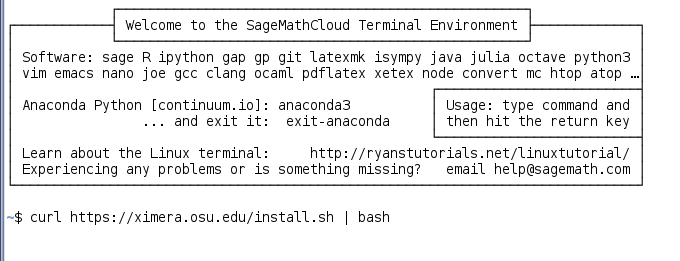
\includegraphics{typingCurl.png}
\end{image}
and you will type:
\begin{verbatim}
curl https://ximera.osu.edu/install.sh | bash
\end{verbatim}
This will install all the required tools (like the Ximera class file,
the `xake' build tool to compile and publish to the server, and mutool
for rasterizing graphics).


\end{document}
